\section{Proposed RPL-ClusterIDS Architecture}
\label{sec:arch}

\subsection{Design Overview}
RPL-ClusterIDS overlays a \emph{logical clustering plane} on top of the physical RPL DODAG.
The routing graph and the security hierarchy are related but not identical: a cluster groups nodes that share local context and can collaborate efficiently, while RPL still determines forwarding parents.
Each node maintains a cluster membership table, a role flag (member or cluster head), and a detection mode selected by the context-adaptive policy engine.

The architecture follows three principles:
\begin{enumerate}
  \item \textbf{Hierarchy without centralization.} Members screen locally; cluster heads analyze regionally; the border router may corroborate network-wide campaigns.
  \item \textbf{Clustering as a resource allocator.} Detection depth and communication budget are allocated where energy, stability, and traffic priority justify them.
  \item \textbf{Explicit security--lifetime trade-off.} When energy is scarce, the system reduces vigilance in a controlled and measurable way rather than failing silently.
\end{enumerate}

Fig.~\ref{fig:arch} summarizes the resulting data and alert paths.

\begin{figure}[!t]
  \centering
  \resizebox{\linewidth}{!}{% Fig. 1 — RPL-ClusterIDS architecture (illustrative).
\begin{tikzpicture}[
  font=\footnotesize,
  node distance=0.55cm and 0.75cm,
  box/.style={draw, rounded corners=2pt, align=center, minimum width=2.35cm, minimum height=0.75cm, fill=gray!8},
  br/.style={box, fill=blue!8},
  ch/.style={box, fill=orange!12},
  mem/.style={box, fill=green!10},
  arr/.style={-{Latex[length=2mm]}, thick}
]
  \node[br] (br) {Border Router\\{\scriptsize optional fusion}};
  \node[ch, below=of br] (ch1) {Cluster Head\\{\scriptsize rules + two-stage verification}};
  \node[ch, left=1.6cm of ch1] (ch2) {Cluster Head};
  \node[ch, right=1.6cm of ch1] (ch3) {Cluster Head};
  \node[mem, below left=0.9cm and 0.1cm of ch1] (m1) {Member\\{\scriptsize rules + LAS}};
  \node[mem, below=0.9cm of ch1] (m2) {Member};
  \node[mem, below right=0.9cm and 0.1cm of ch1] (m3) {Member};
  \node[mem, below=0.9cm of ch2] (m4) {Member};
  \node[mem, below=0.9cm of ch3] (m5) {Member};
  \draw[arr] (m1) -- (ch1);
  \draw[arr] (m2) -- (ch1);
  \draw[arr] (m3) -- (ch1);
  \draw[arr] (m4) -- (ch2);
  \draw[arr] (m5) -- (ch3);
  \draw[arr, dashed] (ch1) -- node[above, font=\scriptsize]{sparse summaries} (ch2);
  \draw[arr, dashed] (ch1) -- (ch3);
  \draw[arr, dashed] (ch1) -- (br);
  \node[below=0.15cm of m2, font=\scriptsize\itshape] {RPL DODAG (underlying routing plane)};
\end{tikzpicture}
}
  \caption{\CaptionFigOne}
  \label{fig:arch}
\end{figure}

\subsection{Dynamic Energy-Context-Aware Clustering}
Clustering is the mechanism that makes hierarchical detection scalable on resource-constrained hardware.
Instead of fixing clusters at deployment time, RPL-ClusterIDS recomputes membership as local context evolves.

\subsubsection{Traffic-priority classes}
Application flows are mapped to four priority classes $C0,\ldots,C3$, where $C0$ denotes background telemetry and $C3$ denotes safety- or control-critical traffic.
This taxonomy modulates IDS vigilance only; it does not alter RPL parent selection~\cite{beno2018qosrpl}.
Each node maintains the fraction of packets observed in each class over a sliding window.
The dominant class in a neighborhood influences how aggressively that region is monitored.

\subsubsection{Cluster affinity and formation}
Each node $i$ evaluates candidate cluster anchors $j$ within two hops using a cluster affinity score:
\begin{equation}
\label{eq:affinity}
\mathcal{A}_{i,j} = w_e \cdot \mathrm{NRE}_j + w_s \cdot \mathrm{Stab}_j + w_t \cdot \mathrm{TC}_j - w_d \cdot \mathrm{Dist}_{i,j},
\end{equation}
where $\mathrm{NRE}_j \in [0,1]$ is normalized residual energy from Energest, $\mathrm{Stab}_j$ is the inverse of parent-change frequency over window $T$, $\mathrm{TC}_j$ is the fraction of $C2$ and $C3$ traffic observed at node $j$, $\mathrm{Dist}_{i,j}$ is hop distance, and weights $w_e,w_s,w_t,w_d$ sum to one (chosen after preliminary sensitivity runs; see Section~\ref{sec:results}).
Node $i$ affiliates with the cluster headed by the feasible neighbor that maximizes $\mathcal{A}_{i,j}$, subject to a cardinality cap that prevents oversized clusters.
Fig.~\ref{fig:cluster-overlay} illustrates how logical clusters relate to the underlying RPL parent graph.

\begin{figure}[!t]
  \centering
  \resizebox{\linewidth}{!}{% Fig. 2 — Cluster overlay on RPL DODAG (illustrative).
\begin{tikzpicture}[font=\footnotesize, scale=0.95, transform shape]
  \node[circle, draw, fill=blue!10, minimum size=6mm] (r) at (0,0) {BR};
  \node[circle, draw, fill=orange!15, minimum size=5mm] (a) at (-1.4,-1.1) {};
  \node[circle, draw, fill=orange!15, minimum size=5mm] (b) at (0,-1.2) {};
  \node[circle, draw, fill=orange!15, minimum size=5mm] (c) at (1.4,-1.1) {};
  \node[circle, draw, fill=green!12, minimum size=4mm] (d) at (-2.1,-2.2) {};
  \node[circle, draw, fill=green!12, minimum size=4mm] (e) at (-0.7,-2.3) {};
  \node[circle, draw, fill=green!12, minimum size=4mm] (f) at (0.7,-2.3) {};
  \node[circle, draw, fill=green!12, minimum size=4mm] (g) at (2.1,-2.2) {};
  \draw[thick, -{Latex}] (r) -- (a); \draw[thick, -{Latex}] (r) -- (b); \draw[thick, -{Latex}] (r) -- (c);
  \draw[thick, -{Latex}] (a) -- (d); \draw[thick, -{Latex}] (a) -- (e);
  \draw[thick, -{Latex}] (b) -- (e); \draw[thick, -{Latex}] (b) -- (f);
  \draw[thick, -{Latex}] (c) -- (f); \draw[thick, -{Latex}] (c) -- (g);
  \draw[dashed, rounded corners=8pt, orange!60] (-2.5,-0.6) rectangle (-0.2,-2.7);
  \draw[dashed, rounded corners=8pt, teal!60] (-0.5,-0.6) rectangle (1.0,-2.8);
  \draw[dashed, rounded corners=8pt, violet!50] (0.8,-0.6) rectangle (2.6,-2.7);
  \node[font=\scriptsize] at (-1.35,-0.35) {Cluster A};
  \node[font=\scriptsize] at (0.25,-0.35) {Cluster B};
  \node[font=\scriptsize] at (1.75,-0.35) {Cluster C};
  \node[font=\scriptsize\itshape] at (0,-2.95) {Solid: RPL parents \quad Dashed: cluster groups};
\end{tikzpicture}
}
  \caption{\CaptionFigTwo}
  \label{fig:cluster-overlay}
\end{figure}

This formulation binds topology, energy, and application priority into a single join decision.
A stable, energy-rich node serving critical traffic becomes a natural cluster anchor, whereas unstable or depleted nodes remain members.

\subsubsection{Context-driven reclustering}
Static clusters become stale as batteries drain and parents change.
The reclustering interval $\Delta_c$ therefore adapts to network condition:
\begin{equation}
\label{eq:recluster}
\Delta_c = \Delta_0 \cdot \bigl(1 + \alpha(1-\overline{\mathrm{NRE}}) + \beta \cdot \mathrm{CtrlLoad}\bigr),
\end{equation}
where $\Delta_0$ is the baseline period, $\overline{\mathrm{NRE}}$ is mean network residual energy, $\mathrm{CtrlLoad} \in [0,1]$ is the normalized control-plane load (ratio of observed DIO/DAO rate to a configured maximum), and $\alpha,\beta$ tune sensitivity.
When $\overline{\mathrm{NRE}} < \tau_{\mathrm{low}}$, clusters merge to reduce the number of cluster heads and associated signaling.
Conversely, in $C3$-dominated regions with healthy energy, clusters may split to improve spatial resolution.

\subsection{Adaptive Cluster-Head Election and Rotation}
Cluster heads perform the most expensive detection work and must therefore be selected from nodes that can sustain the role.
Candidate fitness is defined as:
\begin{equation}
\label{eq:chfit}
\mathcal{F}_j = \lambda_1 \mathrm{NRE}_j + \lambda_2 \mathrm{Stab}_j + \lambda_3 \mathrm{Cent}_j - \lambda_4 \mathrm{Load}_j,
\end{equation}
where $\mathrm{Cent}_j$ is a child-count-based centrality proxy in the DODAG and $\mathrm{Load}_j$ is the current IDS processing load.
Nodes with $\mathrm{NRE}_j < \tau_{\mathrm{CH}}$ are ineligible.
A head retains its role while $\mathcal{F}_j$ remains above a hysteresis threshold and its tenure is below $T_{\max}$.
Rotation prevents long-lived heads from becoming single points of failure and limits the impact of targeted exhaustion attacks against high-fitness nodes.

\subsection{Member-Level Detection: Lightweight Rules and LAS}
Every ordinary member executes four inexpensive rules:
\begin{itemize}
  \item \textbf{R1:} rank increases without corresponding link degradation;
  \item \textbf{R2:} parent-change rate exceeds the neighborhood median by a configurable margin;
  \item \textbf{R3:} DAO transmission rate departs from the local baseline;
  \item \textbf{R4:} downstream gaps appear on $C2$ or $C3$ flows.
\end{itemize}
Each rule produces a weighted flag $r_{i,k}$.
The local anomaly score is:
\begin{equation}
\label{eq:las}
\mathrm{LAS}_i = \sum_{k=1}^{4} \omega_k r_{i,k} \in [0,1], \qquad \sum_{k=1}^{4} \omega_k = 1,
\end{equation}
quantized to four bits before uplink transmission.
Members send LAS summaries to their cluster head every $\Delta_r$ seconds.
The reporting interval is shorter in $C3$-heavy clusters and longer when the node operates in an energy-preserving mode.

This tier keeps per-node computation bounded while ensuring that obvious local deviations are surfaced quickly.

\subsection{Cluster-Head-Level Advanced Detection}
Cluster heads maintain a time-windowed view of member LAS series, neighborhood ETX variance, and control-packet inter-arrival statistics.
A \emph{cluster alert} is raised when any of the following conditions holds:
\begin{enumerate}
  \item at least $\theta_1$ members report $\mathrm{LAS} > \tau_{\mathrm{las}}$ within the same window;
  \item coordinated rank oscillation suggests a distributed rank attack;
  \item a second-stage threshold check confirms the cluster alert when member LAS exceeds $\tau_{\mathrm{ch}} = 0.70$.
\end{enumerate}

The hybrid design is deliberate.
Rules deliver fast, interpretable detection for severe violations, while the second-stage threshold filters false positives without exporting raw packet traces.
Because only cluster heads execute the verification, the additional cost is paid by a small subset of nodes.

\subsection{Limited Inter-Cluster Collaboration}
Unrestricted alert broadcasting would recreate the scalability problems of flat distributed IDS designs.
Cluster heads therefore exchange \emph{cluster summary records} only when cluster-level suspicion exceeds $\tau_{\mathrm{inter}}$.
A summary contains an anonymized cluster identifier, dominant anomaly class, peak LAS aggregate, and timestamp.
Worst-case inter-cluster traffic is $O(K)$ messages per event, where $K$ is the number of cluster heads, rather than $O(N)$ among all nodes.
The border router may fuse summaries from multiple heads when an attack spans cluster boundaries.

\subsection{Context-Adaptive Detection Policy}
The policy engine exposes three operating modes:
\begin{itemize}
  \item \textsc{Full}: all rules and CH threshold verification active; clusters may split for finer coverage; used when energy is ample and $C3$ traffic dominates.
  \item \textsc{Balanced}: default mode; rules R1--R3 active, CH verification invoked on positive rule clusters only.
  \item \textsc{Eco}: triggered when $\overline{\mathrm{NRE}}<\tau_{\mathrm{low}}$ or when more than 40\% of nodes raise battery alarms; rules R3--R4 disabled at members, CH verification suppressed at heads, and $\Delta_c$ doubled.
\end{itemize}
By making this trade-off explicit, RPL-ClusterIDS acknowledges that constrained networks may prefer extended lifetime over maximum detection intensity during benign periods.
Fig.~\ref{fig:policy-weights} summarizes how affinity weights and mode thresholds respond to live context.

\begin{figure}[!t]
  \centering
  \resizebox{\linewidth}{!}{% Fig. 3 — Context policy weights (illustrative).
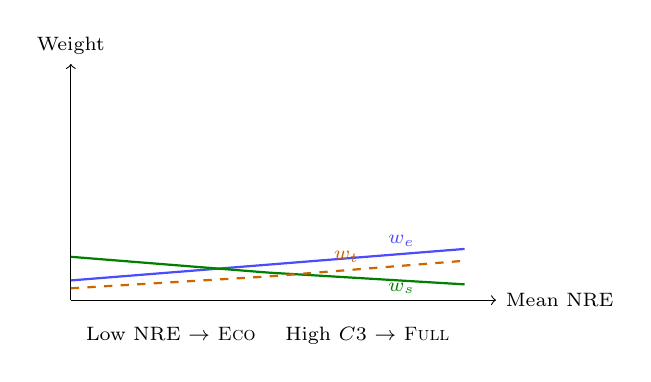
\begin{tikzpicture}[font=\footnotesize]
  \begin{scope}
    \draw[->] (0,0) -- (5.4,0) node[right]{\scriptsize Mean NRE};
    \draw[->] (0,0) -- (0,3.0) node[above]{\scriptsize Weight};
    \draw[thick, blue!70] plot coordinates {(0,0.25) (2.5,0.45) (5,0.65)};
    \draw[thick, green!50!black] plot coordinates {(0,0.55) (2.5,0.35) (5,0.20)};
    \draw[thick, orange!80!black, dashed] plot coordinates {(0,0.15) (2.5,0.30) (5,0.50)};
    \node[blue!70] at (4.2,0.75) {\scriptsize $w_e$};
    \node[green!50!black] at (4.2,0.15) {\scriptsize $w_s$};
    \node[orange!80!black] at (3.5,0.55) {\scriptsize $w_t$};
    \node[font=\scriptsize] at (2.5,-0.45) {Low NRE $\rightarrow$ \textsc{Eco} \quad High $C3$ $\rightarrow$ \textsc{Full}};
  \end{scope}
\end{tikzpicture}
}
  \caption{\CaptionFigThree}
  \label{fig:policy-weights}
\end{figure}

\subsection{Operational Walkthrough}
Consider a 50-node DODAG in which three nodes launch a localized rank attack.
Affected members detect rank and parent-churn anomalies, raising their LAS values.
The cluster head observes correlated LAS spikes across multiple members, confirms the pattern with the second-stage threshold, and emits a cluster alert.
Neighboring heads receive a summary only if the attack begins to spread across cluster boundaries.
If the network enters \textsc{Eco} mode because of low mean NRE, members continue to run R1 and R2 so that severe control-plane attacks remain visible while energy-intensive checks are deferred.
